\documentclass[conference]{IEEEtran}
\IEEEoverridecommandlockouts
% The preceding line is only needed to identify funding in the first footnote. If that is unneeded, please comment it out.
\usepackage{cite}
\usepackage{amsmath,amssymb,amsfonts}
\usepackage{algorithmic}
\usepackage{graphicx}
\usepackage{textcomp}
\usepackage{xcolor}
\def\BibTeX{{\rm B\kern-.05em{\sc i\kern-.025em b}\kern-.08em
    T\kern-.1667em\lower.7ex\hbox{E}\kern-.125emX}}

%=================================================================
%====ADDITIONAL PACKAGES & SETTINGS FROM THE ORIGINAL TEMPALTE====
\usepackage{import} % to use \import{../../../content-tex/}{abstract}
\usepackage{todonotes} % USAGE: \todo[inline]{is there a better example from X topic?}
\usepackage{lipsum}  % USAGE \lipsum[2-4]
\graphicspath{{../figures}} %goes to path: figures/

\begin{document}

\title{
% Diversity, Equity, and Inclusion of Artificial Intelligence and Robotics for children %Fri  7 Jan 23:59:42 GMT 2022
%Piloting Inclusive Workshops of Artificial Intelligence and Robotics for children %Sat  8 Jan 00:12:35 GMT 2022
%Piloting Inclusive Artificial Intelligence and Robotics for Children %Sat 15 Jan 08:44:06 GMT 2022
%Piloting Diversity and Inclusion in Artificial Intelligence and Robotics for Children %Sat 15 Jan 10:33:54 GMT 2022
Piloting Diversity and Inclusion Workshops in Artificial Intelligence and Robotics for Children %Sun 16 Jan 13:14:45 GMT 2022
}

\author{

\IEEEauthorblockN{1\textsuperscript{st} AIR4Children}
\IEEEauthorblockA{\textit{dept. name of organization (of Aff.)} \\
\textit{air4children: Artificial Intelligence and Robotics}\\
Xicohtzinco, M\'exico \\
air4children@gmail.com}

}

% \author{\IEEEauthorblockN{1\textsuperscript{st} Given Name Surname}
% \IEEEauthorblockA{\textit{dept. name of organization (of Aff.)} \\
% \textit{name of organization (of Aff.)}\\
% City, Country \\
% email address or ORCID}
% \and
% \IEEEauthorblockN{2\textsuperscript{nd} Given Name Surname}
% \IEEEauthorblockA{\textit{dept. name of organization (of Aff.)} \\
% \textit{name of organization (of Aff.)}\\
% City, Country \\
% email address or ORCID}
% \and
% \IEEEauthorblockN{3\textsuperscript{rd} Given Name Surname}
% \IEEEauthorblockA{\textit{dept. name of organization (of Aff.)} \\
% \textit{name of organization (of Aff.)}\\
% City, Country \\
% email address or ORCID}
% \and
% \IEEEauthorblockN{4\textsuperscript{th} Given Name Surname}
% \IEEEauthorblockA{\textit{dept. name of organization (of Aff.)} \\
% \textit{name of organization (of Aff.)}\\
% City, Country \\
% email address or ORCID}
% \and
% \IEEEauthorblockN{5\textsuperscript{th} Given Name Surname}
% \IEEEauthorblockA{\textit{dept. name of organization (of Aff.)} \\
% \textit{name of organization (of Aff.)}\\
% City, Country \\
% email address or ORCID}
% \and
% \IEEEauthorblockN{6\textsuperscript{th} Given Name Surname}
% \IEEEauthorblockA{\textit{dept. name of organization (of Aff.)} \\
% \textit{name of organization (of Aff.)}\\
% City, Country \\
% email address or ORCID}
% }

\maketitle

\begin{abstract}
This document is a model and instructions for \LaTeX.
This and the IEEEtran.cls file define the components of your paper [title, text, heads, etc.]. 
*CRITICAL: Do Not Use Symbols, Special Characters, Footnotes, or Math in Paper Title or Abstract.
\lipsum[2]
\end{abstract}

\begin{IEEEkeywords}
component, formatting, style, styling, insert
\end{IEEEkeywords}

%%%%%%%%%%%%%%%%%%%%%%%%%%%%%%%%%%%%%%%%%
%%%%%%%%%%%%%%%%%%%%%%%%%%%%%%%%%%%%%%%%%
\section{Introduction}
Guarantey security, accessibitly and human dignity can be considered the pilar for inclusivity.
However, the disparity of advances in education and technology is not creating enviroments to construct a faier society.
Recently, Astobiza et al. reported the need of collaborations between industry and a multidisiplanry gropu of reserachers to address concernts on the paradigm of inclusivity in robotics \cite{MonasterioAstobiza2019}.
Simiarly, Astobiza et al. suggested that inclusive robotics should be based on: "1) they should be easy to use and 2) they must contribute to making accessibility easier in distinct environments" \cite{MonasterioAstobiza2019}.
Peixoto et al. in 2018 reported the use of robots as tool to promote diverity which lead to improve competences in communication, teamwork, leadhership, problem solving, resilence and entrreprenurship \cite{PeixotoCastro2018, PeixotoGonzalez2018}. 
Pannier et al. pointed out the challenges of increasing the  participation of women and underrepresented minorities in the areas of Mechatronics and Robotics Engineering as well as the creation of community of educators to promote diversity and inclussion \cite{Pannier2020}.
Pannier et al. mentioned that the prevalence of free and open-source software and hardware made mechatronics more accesible to a diverse group of population \cite{Pannier2020}.
Also, Pannier et al touched on the evidence and importance of offering workshops to different ragne of underpresentend students that lead to inpires other programs to creat outreach activities for studnets, trainings, workshops, 

This short paper presents our findinds on the first pilot workshop to promote diversity and inlcusion in Artificial Intelligence and Robotics.


%%%%%%%%%%%%%%%%%%%%%%%%%%%%%%%%%%%%%%%%%
%%%%%%%%%%%%%%%%%%%%%%%%%%%%%%%%%%%%%%%%%
\section{Diversity and Inclusivity of AIR4children with Non-tradional Education}

\subsection{Alternative education programs}
Alternative education programs such as Montessori, Waldorf and Regio Emilia considers children as active authors of their own development \cite{edwards2002}.
Such programs that in a way follow same phylosofies have been adopted internationally.
However the contributes changes of technologies have been started to evolve. 
For instnace, Edwards pointed out the schools deriving from the same phylosogy might also need to obsersve teacher-child interactions, its enviroments and interview to the past and present parents and children \cite{edwards2002}
Recently, Aljabreen pointed out the adoptions of new technologies and how early child educatio is re-conceptualised \cite{Aljabreen2020}.

\subsection{Montesory education}
Elkin et al. in 2014 explored the how robots can be used in the Montessori curriculum \cite{elkin2014}.
Authors conclude that the confidence and experience in robotics is crucial to deliver and communicate the right experince to encourgage students \cite{elkin2014}.
Similry Elkin et al. posed the question on the revision of new curriculums of technology that do not deviate from the purpose of the Montesory classrom \cite{elkin2014}.
Drigas and Gkeka in 2016 reviewed the application of information and communication technologes in the Montesory Method \cite{DrigasGkeka2016}.
Drigas and Gkeka mentioned the Manipulatives, as objects to develop motor skills or understan mathematical abstractions, are based on cultural areas, language, mathemaics and sensorial but little to none on technolgoical areas.
Drigas and Gkeka reviewed Montesory materials of the 21st century where interactive systems with sounds and lights, touch application to enhace visual literacy or the development of compuitational thinking and contrictuons of the physical world \cite{DrigasGkeka2016}
These indicate that the incorporation of such manipulatives with the use of robotics might led to reach scneraios to explore motor skill develipment, visualisation and computational thikning. 

Recenlty, Scippo and Ardolino reported a longitudinal study of the use of computationla thinking in five years participants of primary shcool in a Montessori school \cite{ScippoArdolino2021}
Scippo and Ardolino pointed out the importance of aligment of the Montessori material with the computationla thinking acitivites. 

\subsection{Other alternative education styles}
Synthesis is new education program, started in 2014 with Josh Dahn and support of Elon Musk, which aim is to cultivate student voice, strategic thinking and collaborative problem solving \cite{synthesis2022}.

%%%%%%%%%%%%%%%%%%%%%%%%%%%%%%%%%%%%%%%%%
%%%%%%%%%%%%%%%%%%%%%%%%%%%%%%%%%%%%%%%%%
\section{Designing Diversity and Inclusion  Workshops}
Considering the challenges of low-to-middle-income countries faces, technologies such as robotics and artitificial intelligence might not be avaialble to towns. 
In that sense, we focos this work on a pilot experiment to promote diverity of and inclusion to children to teach AI and Robotics. 

\paragraph{Lesson 01: Braking the ice and motivations} 
Place figures and tables at the top and bottom of columns. Avoid placing them in the middle of columns. 
Large figures and tables may span across both columns. Figure captions should be below the figures; table heads should appear above the tables. 
Insert figures and tables after they are cited in the text. Use the abbreviation 

\paragraph{Lesson 02: Human senses and coding my first robot} 
Place figures and tables at the top and bottom of columns. Avoid placing them in the middle of columns. 
Large figures and tables may span across both columns. Figure captions should be below the figures; table heads should appear above the tables. 
Insert figures and tables after they are cited in the text. Use the abbreviation 

\paragraph{Lesson 03: Playing with reaction-action activities} 
Place figures and tables at the top and bottom of columns. Avoid placing them in the middle of columns. 
Large figures and tables may span across both columns. Figure captions should be below the figures; table heads should appear above the tables. 
Insert figures and tables after they are cited in the text. Use the abbreviation 

\paragraph{Lesson 04: Develop your own AIR} 
Place figures and tables at the top and bottom of columns. Avoid placing them in the middle of columns. 
Large figures and tables may span across both columns. Figure captions should be below the figures; table heads should appear above the tables. 
Insert figures and tables after they are cited in the text. Use the abbreviation 

Figure \ref{fig:curriculum} presents four lessons of the workshops.
\begin{figure}[htbp]
    \centerline{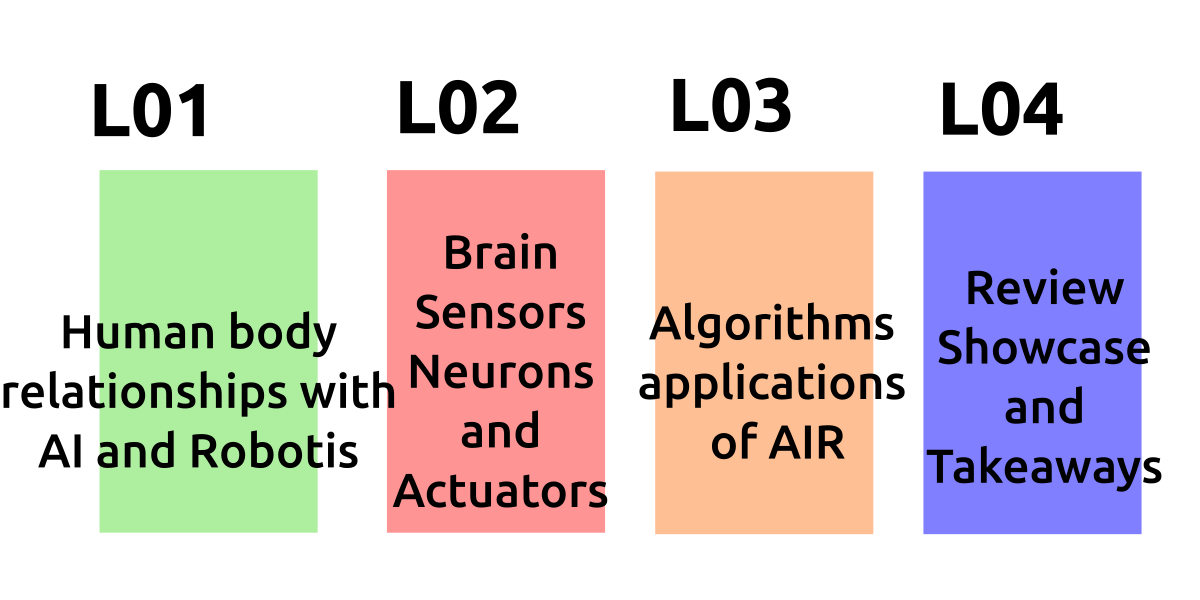
\includegraphics[width=\linewidth]{curriculum-design/versions/drawing-v00.png}}
    \caption{Curriculum for four lessons (L01 to L04). 
    Lesson 01 introduce the course, 
    lesson 02 provides the basics of anatomy, 
    lesson 03 covers algorihtms, and 
    lesson 04 wraup and showcase the project of children.
    }
    \label{fig:curriculum}
\end{figure}

%%%%%%%%%%%%%%%%%%%%%%%%%%%%%%%%%%%%%%%%%
%%%%%%%%%%%%%%%%%%%%%%%%%%%%%%%%%%%%%%%%%
\section{Piloting Diversity and Inclusion Workshops}
We invited 14 particpants (six female and eight male) with range of age from 6 to 11 years old (average age of 7.64).
Three instructors and two coordinators delivered four lessons. 
Each lessons lasted 90 minutes with breaks of 15 minutes at the middle of each lesson. 
Figure \ref{fig:pilot} illustrates instructors and children intercting with activities. 
\begin{figure}[htbp]
    \centerline{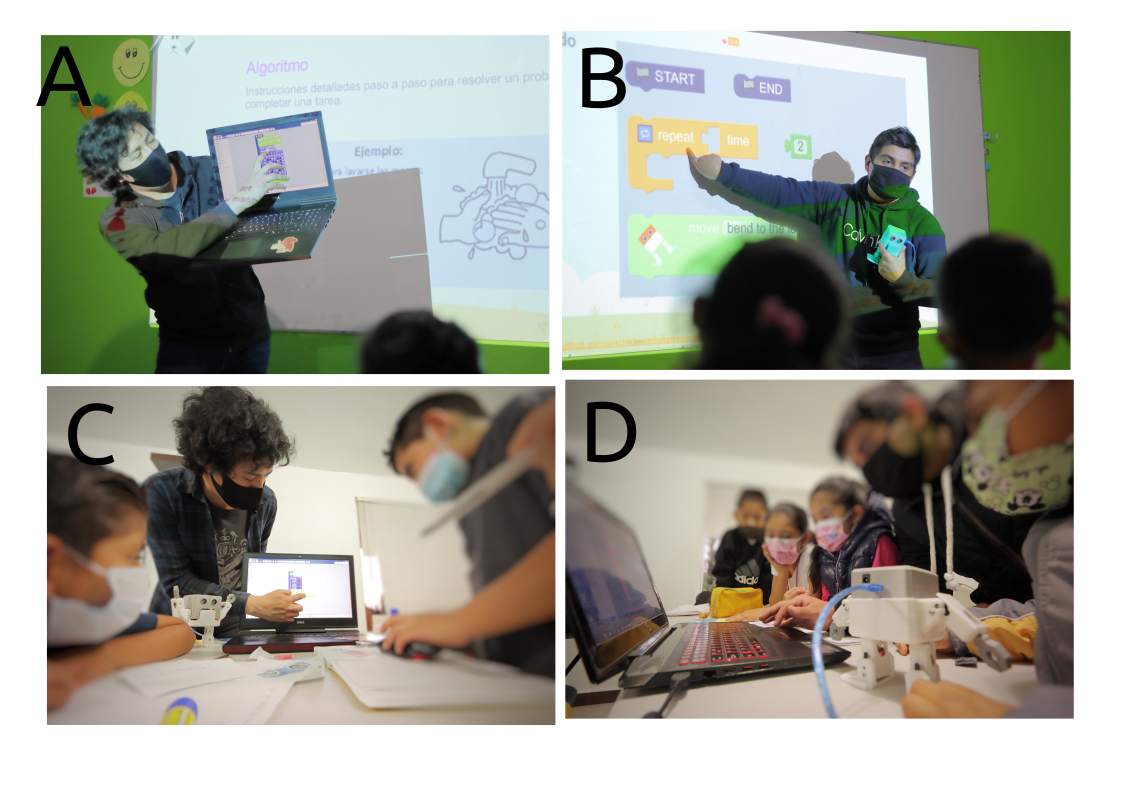
\includegraphics[width=\linewidth]{piloting-workshops/versions/drawing-v00.png}}
    \caption{Instructors demonstrating basics of AI and Robotics. 
    Children engaging with robots, classmates and instructors.}
    \label{fig:pilot}
\end{figure}


\begin{table}[htbp]
    \caption{Table Type Styles}
    \begin{center}
    \begin{tabular}{|c|c|c|c|}
    \hline
    \textbf{Table}&\multicolumn{3}{|c|}{\textbf{Table Column Head}} \\
    \cline{2-4} 
    \textbf{Head} & \textbf{\textit{Table column subhead}}& \textbf{\textit{Subhead}}& \textbf{\textit{Subhead}} \\
    \hline
    copy& More table copy$^{\mathrm{a}}$& &  \\
    \hline
    \multicolumn{4}{l}{$^{\mathrm{a}}$Sample of a Table footnote.}
    \end{tabular}
    \label{tab1}
    \end{center}
\end{table}
    


%%%%%%%%%%%%%%%%%%%%%%%%%%%%%%%%%%%%%%%%%
%%%%%%%%%%%%%%%%%%%%%%%%%%%%%%%%%%%%%%%%%
\section{Conclusions and future work}
A pilot workshop to promoto diversity and inclusion to teach AI and Robotics to 14 children was successfully organised in Xicohtzinco Mexico last Novemeber 2021.
In such workshop, activiites were designing to encougage particpantes to engage with each other. 
Similarly, the workshops were free cost to encongrage particpation of anyone. 
We realised that grouping children with four participans was challenging because of the space as well as having a more engaging interaction with the subjects of the group. 
That said, we are planing to organise another workshop in third quatiremster of 2022 where lessons will be better organised, material will combine more interactive activitie and robots and material will be suited for three particants per group. 

\section*{Acknowledgment}
To Rocio Montenegro for her contributions with the design of the Montessori curriculum for the workshops.
To Marta P\'erez, for their support in organising the pilot of the workshops.
To Diego Donato Badillo-Per\'ez and Antonio Badillo-Per\'e\ for voluntering as instructors of the workshops.
To Leticia V\'azquez for her support with the logistics and feedback to improve the workshops.
To Elias Mendes for his support and feedback on the hardware design of the robot.
To Dago Cruz for his contributions on open source AI and Robotics.
To Angel Mandujano, Elva Corona and others who have contributed with feedback and support to keep reitering the project of AIR4children. 

\bibliographystyle{IEEEtran}
\bibliography{../references/references}

\end{document}
